\documentclass{article}

%PACKAGES
\usepackage[utf8]{inputenc}
\usepackage{natbib}
\usepackage{graphicx}
\graphicspath{ {./Figures/} }
\usepackage{amsmath} % \vspace{} \hspace{}
\usepackage{physics}
\usepackage[margin=3cm]{geometry}
\usepackage{textpos} % plaats vakje voor figures
\usepackage{float} % Voor H! gebruik in figures
\usepackage{caption} 
\usepackage{changepage} % Changes table to left
\usepackage{comment}% Includes \begin{comment}
\usepackage{fancyhdr}
\usepackage{url}
\pagestyle{fancy}
\usepackage{xcolor} % colorpackage
\usepackage[colorlinks,linkcolor=black, citecolor=teal,urlcolor=blue]{hyperref} % hyperlinks citations
\usepackage{amssymb} % Expected symbol (\mathbb{E})
\usepackage{algorithm} % implement algorithm pseudocode
\usepackage{subcaption} % For multiple images
% \usepackage{subfigure}
\usepackage{bm} % For \boldsymbol
\usepackage{amsmath}

%NEW COMMANDS
\newcommand{\eg}{e.\,g.\ }
\newcommand{\ie}{i.\,e.\ }

\newcommand{\WeightVector}{\overset{\rightarrow}{\boldsymbol{\theta}} }

%BEGIN DOCUMENT
\begin{document}
\nocite{*} % dont order citations

\thispagestyle{empty} 
\begin{center}
    \vspace*{0.5cm}
    \huge
    \textbf{SOLVING THE ART GALLERY PROBLEM USING GRADIENT DESCENT}

    \vspace*{0.4cm}
    \textbf{Thesis Proposal }
    \vspace*{2cm}

    % \begin{figure}[H]
    %     \centering   
    %     
\includegraphics[width = 11cm]{Figures/titlepage robot computer slither.png}
    % \end{figure}


    %Req indent

    \vspace{-1cm}
    \LARGE
    Georgiana Juglan
    \vfill 
    \large    
    \textbf{Supervisor:} \\
    Tillmann Miltzow \\
    \textbf{Second Examiner:} \\
    Frank Staals \\
     
\end{center}
   

\begin{textblock}{3}(6.5,0.7)

\includegraphics[width = 6cm]{Figures/UU logo.png}
\end{textblock}

\begin{flushleft}
    \vspace{0.5cm}
    Master's Thesis \\
    Computing Science\\
    \today\\
    Student Nr. 2996307 \\
    Utrecht University\\
    The Netherlands
\end{flushleft}

\newpage
\thispagestyle{empty}
\section*{Abstract}

% In this thesis, machine learning agents learn to play the online browser game \href{https://Slither.io}{Slither.io}. In \textit{Slither} you play as a snake where the goal is to grow, by killing other snakes and eating food pellets. There are over 100 snakes in a single arena, and every player competes against each other under the same circumstances. The game has simple rules and controls, and yet complicated situations constantly emerge. The agents are trained with multiple machine learning methods such as imitation learning and deep Q-learning. Actor-critic policy gradient methods like PPO and SAC are given special attention, as they have the greatest potential in training agents that achieve superhuman performance. If time allows, the more complicated model-based methods are explored. The agents can observe their environment in different ways. For example by passing visual images through a CNN. This training and observing is established with an in-house replica of Slither in the game-engine Unity. Unity uses an API for communication with Python's machine learning library PyTorch to implement the machine learning algorithms. The main goal of this thesis is to create a superhuman player in Slither which can be deployed onto the original browser game.  Additionally, the aim is to compare the performance of different algorithms and techniques, to better understand how to effectively and efficiently train agents on competitive video games.

The Art Gallery Problem is one of the central problems in computational geometry. It was recently shown that the problem is $\exists \mathbb{R}$-complete. Thus it is unlikely to be solvable by methods that are usually applied to NP-complete problems. These methods include heuristics with provable guarantees to come as close as possible to the optimal solution in polynomial time. Nonetheless, one of the most important methods to solve $\exists \mathbb{R}$-complete problems is called gradient descent. Curiously, there was no attempt yet to solve the Art Gallery Problem by gradient descent. By aiming to maximise the area seen by the guards in the Art Gallery Problem, we get a continuous cost function, which allows us to compute a gradient. Using the gradient and other heuristics inspired from neural networks, we will try to solve the Art Gallery Problem practically using gradient descent. Specifically, we aim to use the library CGAL. 
% Furthermore, we want to use specific data structures to compute the gradient quickly. 
Implementations will show how feasible this approach is. We will visualize the results and discuss the performance of the algorithm on different input shapes and sizes.
\thispagestyle{empty}
\tableofcontents
\thispagestyle{empty}

\section{Literature Summaries}
\subsection{Efficient Computation of Visibility Polygons \cite{DBLP:journals/corr/BungiuHHHK14}}
This paper \cite{DBLP:journals/corr/BungiuHHHK14} introduces the implementations and their experimental evaluations for two existing algorithms (\cite{joe1987corrections}, \cite{asano1985efficient}) and a newly developed one for computing visibility in polygons. These implementations are available in the CGAL library\footnote{\url{https://www.cgal.org/}}, starting with version 4.5.

Working with the visibility region is a basic tool in computational geometry, specifically in the Art Gallery Problem \cite{o1987art}. The Art Gallery Problem \cite{o1987art} is an $\exists \mathbb R$-complete problem \cite{abrahamsen2021art}. The problem class $\exists \mathbb R$ consists of instances that can be reduced in polynomial time to a decision problem of whether a system of polynomial equations with integer coefficients and any number of real variables has a solution. Since NP $\subseteq \exists \mathbb R$, the $\exists \mathbb R$ class is an even harder to solve complexity class, since $\exists \mathbb R$ problems do not admit solutions in polynomial time. For this reason, it is crucial that the computation time of the visibility region is efficiently implemented. 

Therefore, this paper presents 3 algorithms and their implementations' performance.

\subsubsection{Algorithm of Joe and Simpson \cite{joe1987corrections}}
The algorithm of Joe and Simpson \cite{joe1987corrections} runs in $O(n)$ time and space. It begins by sequentially scanning the boundaries of the simple polygon $\mathcal P$, and adds its boundary points $v_i, \forall i = \overline{1, n}$, with $n$ the number of vertices in $\mathcal P$, to a stack $s$. For each processed edge $\overline{v_iv_{i + 1}}$, its endpoints $v_i$ and $v_{i + 1}$ are checked whether they are in the visibility region of the viewpoint $p$. If they are, $v_i$ and $v_{i + 1}$ are added to $s$. Otherwise, they are skipped. At every moment, the algorithm checks whether $\overline{v_iv_{i + 1}}$ obscures a previously added line segment. If that is the case, then the endpoints of the obscured line segment are declared obsolete and deleted. 

% The implementation of the algorithm handles the previously discussed cases for an arrangement $\mathcal P$, while also accounting for the case in which the polygon winds more than 360$^\circ$ using a winding counter.
% - **Algorithm of Joe and Simpson** $O(n)$ time and space
	% - performs a sequential scan of the boundary of $\mathcal P$ and uses a stack $s$ of boundary points $s_0, s_1, ..., s_ as summarised in the following subsections.der to deal with cases in which the polygon winds more than 360*, a winding counter is used during this edge processing
% he points that are visible from $q$ form the visibility region $\mathcal V(q)$ (polygon)

\subsubsection{Algorithm of Asano \cite{asano1985efficient}}
The algorithm of Asano \cite{asano1985efficient} runs in $O(n \log n)$ time and $O(n)$ space and uses a plane sweep approach with event line $L$. It begins by efficiently sorting all the vertices of $\mathcal P$ based on their polar angles with respect to the viewpoint $p$. For example, suppose $p$ and some given points $a_1, a_2, b_1, b_2$ are given in a plane with positive coordinates, as placed in Figure \ref{fig:asano}. The figure is taken from \cite{DBLP:journals/corr/BungiuHHHK14} and annotated in order to facilitate the explanations given in these summaries. Then, the points will be treated in the order of $b_2, b_1, a_2, a_1$ with respect to $p$ and their angular comparisons $\measuredangle b_2Oq < \measuredangle b_1Oq < \measuredangle s_1Oq < \measuredangle a_1Oq$, where $O(0, 0)$. Then, the event line $L$ starts sweeping around $p$. Every line segment that $L$ intersects is stored in a balanced binary tree $T$ in the order of intersection. As $T$ is updated, a new vertex of $\mathcal V(p)$ is stored each time the segment closest to $p$ in $T$ changes. It is important to mention that the intersection between $L$ and line segments is not explicit, but is instead determined by comparisons between the endpoints' coordinates. For instance, in Figure \ref{fig:asano}, the endpoint $b_2$ of line segment $\overline{b_2a_2}$ is the first one $L$ intersects. $b_2$ is thus added to $T$. Then, $L$ continues sweeping and adds $b_1, a_2$ and $a_1$ to $T$. Although $\overline{b_2a_2}$ and $\overline{b_1a_1}$ represent line segments $s_2$ and $s_1$, respectively, the intersection of $L$ with them is not explicitly computed, but is determined based solely on the positions of their endpoints: $s_1$ is farther away from $p$ because $q, a_2$ and $b_2$ are on the same side of $s_2$.

\begin{figure}[h!]
	\centering
	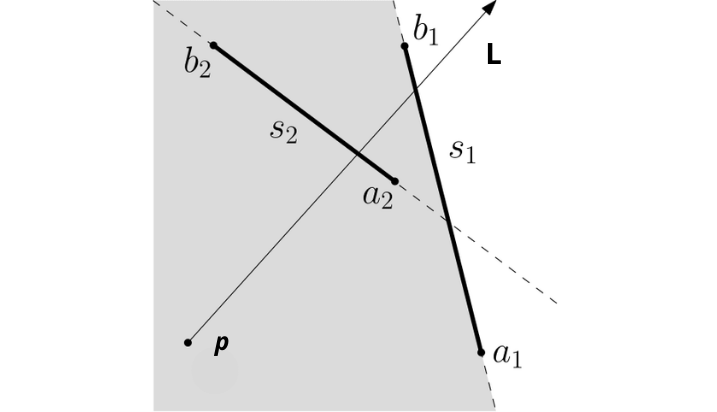
\includegraphics[width = 0.5\textwidth]{compare_segments.png}
	\caption{The Algorithm of Asano \cite{asano1985efficient} Visual Example \cite{DBLP:journals/corr/BungiuHHHK14}.}
	\label{fig:asano}
\end{figure}
	% - as the sweep proceeds, $T$ is updated and a neq vertex of $V(q)$ is generated each time the smallest element (segment closest to $q$) in $T$ changes
	% - important to have efficient comparison ops (e.g.: *add pic*)

\subsubsection{New Algorithm: Triangular Expansion}
The algorithm introduced in the paper is named Triangular Expansion and runs in $O(n^2)$ time and $O(n)$ space. It begins by triangulating $\mathcal P$ in $O(n \log n)$ time if $\mathcal P$ has holes, and $O(n)$ otherwise. Unfortunately the runtime is constrained by CGAL, which makes use of the Delaunay triangulation algorithm \cite{delaunay1934sphere} with $O(n^2)$ time for the worst case, but with better performance in practice. 

Taken from \cite{DBLP:journals/corr/BungiuHHHK14} and annotated to suit the explanations in these summaries, Figure \ref{fig:triangular} depicts an example run of the algorithm on a polygon with holes $\mathcal P$. Starting from the viewpoint $p$, the triangle containing $p$ is located by performing a simple walk. Trivially, $p$ sees the entire triangle it is contained in. The algorithm continues by recursively expanding the view of $p$ from one triangle into the other, until there are no more triangles to expand into. The view of $p$ becomes restricted by the reflex vertices $l$ and $r$ of the third triangle entered by the recursive step. Since $l$ and $r$ are reflex vertices, the view past them is further restricted until the boundaries $l'$ and $r'$ of $\mathcal P$, respectively,  are reached. Line segments $\overline{ll'}$ and $\overline{rr'}$ are added to $\mathcal V(p)$ in their angular order around $p$. At the end, $\mathcal V(p)$ will contain the segments delimiting the visibility polygon of $p$.

\begin{figure}[h!]
	\centering
	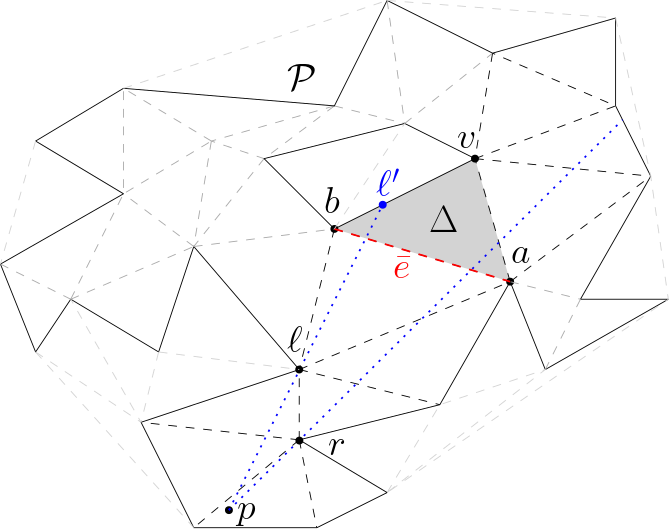
\includegraphics[width = 0.5\textwidth]{triangular_expansion.png}
	\caption{The Triangular Expansion Algorithm Example - recursion entering triangle $\Delta$ through edge $e$ \cite{DBLP:journals/corr/BungiuHHHK14}.}
	\label{fig:triangular}
\end{figure}
% - **triangular expansion** - $O(n^2)$
	% - preprocessing: triangulation ($O(n)$ for simple polygons, $O(n\log n$) for polygons with holes; Delaunay ($O(n^2)$) used)
	% - given $q$, locate the triangle containing $q$ by a simple walk ($q$ sees the entire triangle)
	% - recursive procedure that expands the view of $q$ through that edge into the next triangle. Initially, the view is restricted by the 2 endpoints of the edge, and then further as recursion continues: *add pic* for triangle $\Delta$, the view of $q$ is restricted by the 2 reflex vertices $l$ and $r$ with $a \leq r < l \leq b$ w.r.t. angular order around $q$. $v$ is a new vertex and its position w.r.t. $l$ and $r$ is computed with 2 orientation tests *add pic*: $e_l$ is a boundary edge and we can report edge $\overline{ll'}$ and $\overline{l'v}$ as part of the visibility region of $q$; $e_r$ is not a boundary edge => the recursion continues with $v$ being the vertex that now restricts the left side of the view
	% - the recursion may split into 2 calls if $e_l$ and $e_r$ are both not part of the boundary. As there are $n$ vertices, this can happen $O(n)$ times => worst-case $O(n^2)$; however a true split into two visibility cones that may reach the same triangle independently can only happen at a hole of $\mathcal P$, thus at worst the runtime is $O(nh)$, where $h$ = number of holes (linear time of simple polygons) (e.g.: worst-case *add pic*)
	% - triangulation has linear size, at most $O(n)$ recursive calls on the stack => $O(n)$ space

\subsubsection{Experiments}
The paper does not report on benchmarks with query points on edges in the interior polygon, as it claims that the implementations perform similarly to other already implemented algorithms. Instead, it uses two real-world scenarios (a simple polygon of Norway with 20981 vertices, and a cathedral polygon with 1209 vertices) and a worst-case polygon for the Triangular Expansion algorithm.

In terms of results on the real-world polygons, the Triangular Expansion algorithm has a 2-factor improved performance when compared to Asano's algorithm \cite{asano1985efficient}, and performs one order of magnitude faster than Joe and Simpson's algorithm \cite{joe1987corrections}. For the worst-case scenario, Asano's algorithm \cite{asano1985efficient} outperforms the Triangular Expansion algorithm with increasing input complexity.

Thus, despite the Triangular Expansion algorithm being outperformed in the worst-case scenario, this paper adds efficient implementations for  3 different  polygon visibility algorithms in the CGAL library. The choice of algorithms when using the library can be adapted based on the input polygons. 
% - experiments - no reports on similar benchmarks with query points on edges and in the interior polygon; for the input graphs used, the triangular expansion is 2-factor faster than Asano, and one order of magnitude faster than Joe and Simpson; with increasing input complexity, Asano does become faster
\subsection{Irrational Guards Are Sometimes Needed \cite{abrahamsen2021art}}
This paper \cite{abrahamsen2021art} studies the placement of the guards in the context of The Art Gallery Problem \cite{o1987art}. Namely, it focusses on and confirms that there are polygons with integer coordinates that require guards placed at points with irrational coordinates. Generalising, this paper shows that $\forall n \in \mathbb N$, there is a family of simple monotone polygons that can either be guarded by $3n$ guards with irrational coordinates, or $4n$ guards with rational coordinates. The result is also extended to a rectilinear polygon that can be guarded by 9 guards with irrational coordinates, or 10 guards with rational coordinates. The family of simple monotone polygons that can be guarded by $3n$ guards with irrational coordinates, as well as the rectilinear polygon that can be guarded by 9 guards with irrational coordinates are also discussed.


At the time of writing the paper, there was no combinatorial algorithm for finding an optimal solution for The Art Gallery Problem \cite{o1987art}, nor for its decidability version on whether a set $S$ of given size $k$ exists. As such, it is not known whether the problem is in NP.

First, we will address the question regarding whether polygons given by integer coordinates require guard positions with irrational coordinates in any optimal solution by introducing such a monotone polygon $\mathcal P$. A polygon is monotone if there exists a line $l$ such that every line orthogonal to $l$ intersects it at most twice. $\mathcal P$ is depicted in Figure \ref{fig:p} and is constructed using a rectangle, six triangular pockets (in green), three rectangular pockets (in blue) and four quadrilaterial pockets (in red) are added. The intuition behind the polygon will be explained in the upcoming subsections.

\begin{figure}[h!]
    \centering
    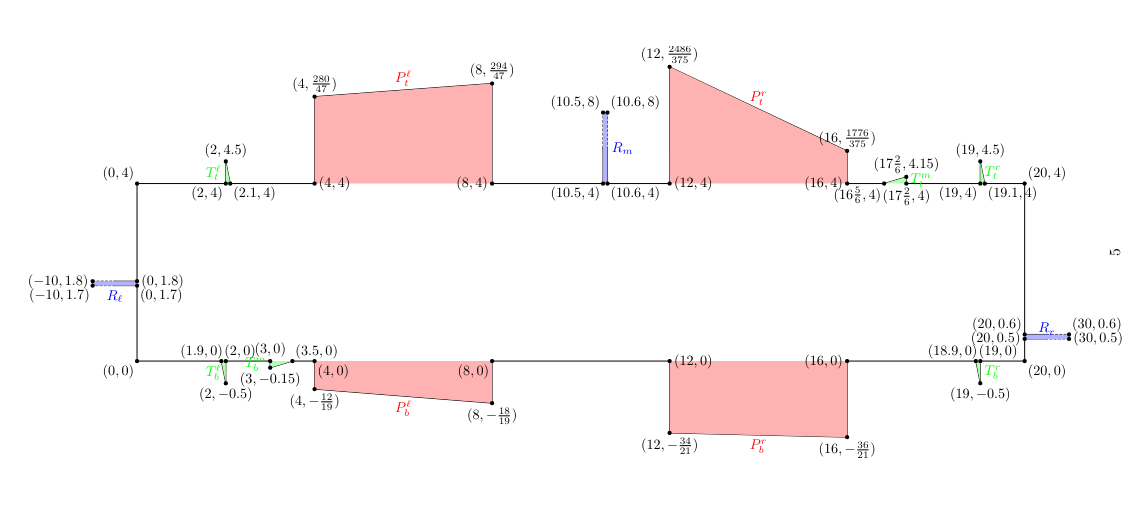
\includegraphics[width=\textwidth]{Screenshot from 2022-01-21 11-17-41.png}
    \caption{Polygon $\mathcal P$}
    \label{fig:p}
\end{figure}

\subsubsection{Intuition for Triangular Pockets}
The six triangular pockets are created in order to force a guard on a line segment. As such, they are grouped into three pairs: top pockets are paired with bottom pockets corresponding to their position in $\mathcal P$. A depiction of this positioning can be found in Figure \ref{fig:tb} (b). For every pair (leftmost, middle, rightmost) of triangular pockets, there is a corresponding line $l_\ell, l_m, l_r$, respectively, that joins the peaks of each triangular pocket in a pair. A guard can see both the peaks $t, b$ of the pockets only if it is placed on the line segment $\overline{tb}$ (Figure \ref{fig:tb} (a)). Hence, one guard is needed per pair, so 3 guards are needed in this case.

\begin{figure}[h!]
    \centering
    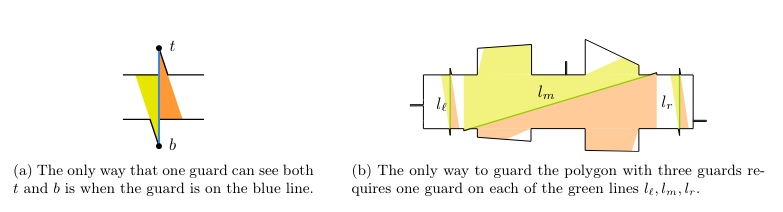
\includegraphics[width=\textwidth]{Screenshot from 2022-02-02 09-57-44.png}
    \caption{Forcing Guards to Lie on Specific Line Segments.}
    \label{fig:tb}
\end{figure}

\subsubsection{Intuition for Quadrilaterial Pockets}
The four quadrilateral pockets are created in order to force a guard in a region bounded by a curve. Figure \ref{fig:quadrilateral_pockets} depicts the visualisation for this case. Considering the fixed position of a guard $g_m$ either on the left or on the right of the curve $c_\ell$, there exists a position of guard $g_\ell$ on $l_\ell$ such that edge $e_t^\ell$ and line $p_b^{\ell}g_m$ are seen by $g_\ell$. Then, only if $g_m$ is on the left or on $c_\ell$ can it see the remaining parts of the pockets that are not seen by $g_\ell$ (edge $e_b^{\ell}$, line $p_t^{\ell}g_{\ell}$). Analogously, in order for the right side of $\mathcal P$ and the right pair of quadrilateral pockets to be seen by both guards $g_m$ and $g_r$, $g_m$ has to be on the curve $c_r$ or on its right. Since $g_m$ has to also satisfy its position on $c_\ell$, its only feasible position is as the intersection point between $c_\ell$ and $c_r$. 

\begin{figure}[h!]
    \centering
    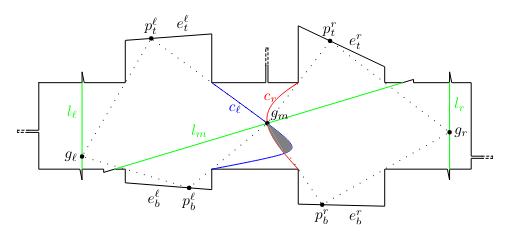
\includegraphics[width=0.7\textwidth]{Screenshot from 2022-01-21 12-02-44.png}
    \caption{Restricting a Guard to a Region Bounded by a Curve}
    \label{fig:quadrilateral_pockets}
\end{figure}

\subsubsection{Intuition for Rectangular Pockets}
The three rectangular pockets are created in order to force a guard to a single irrational point. Further building onto the previously discussed instance from Figure \ref{fig:quadrilateral_pockets}, the three rectangular pockets on the laterals and top of $\mathcal P$ are added.  They then allow for additional constraints for the positions of the guards $g_\ell, g_m, g_r$. Based on the curve equations of $c_\ell$ and $c_r$, we can thus calculate the irrational position of $g_m = (3.5 + 5\sqrt 2, 1.5\sqrt 2)$. Subsequently, we can fix the positions of $g_\ell$ and $g_r$ on lines $l_\ell$ and $l_r$.

\subsubsection{Monotone Polygon Creation}
The polygon $\mathcal P$ in question  was then found through experimentation in GeoGebra\footnote{\url{https://www.geogebra.org/}}. The triangular and rectangular pockets were fixed. Finding then the position of the rectangular pockets required the existence of a rational line that contained the irrational coordinates of guard $g_m$ from Figure \ref{fig:quadrilateral_pockets}. The irrational coordinates of the two other guards $g_\ell, g_r$ were chosen such that they would be able to see the rest of the polygon that is unseen by $g_m$. The rectangular pockets were added based on their coordinates.

In this way, dependencies between guard positions were created with each guard placed on each of the lines $l_\ell, l_m, l_r$ at unique irrational positions. The guard set becomes thus $S = \{g_\ell, g_m, g_r\}$.  Given the properties of the positions of the guards (unique and irrational), the only method to seeing the whole polygon $\mathcal P$ using guards with rational positions would be to use more than 3 (at least 4). This statement can also be generalised such that a family of polygons $(\mathcal{P}_n)_{n \in \mathbb{Z}_+}, \forall n$ can be guarded by $3n$ guards with irrational coordinates, or $4n$ guards with rational coordinates. The coordinates determining the polygons are hence polynomial in $n$.

\subsubsection{Rectilinear Polygon Creation}
Similarly, a rectilinear polygon $\mathcal P_R$ can be created given integer coordinates. $\mathcal P_R$ would require guards with irrational coordinates in any optimal solution. It can be guarded by 9 guards if guards can be placed at points with irrational coordinates. Otherwise, the smallest optimal guard set $S$ with rational coordinates would be of size 10.

$\mathcal P_R$ can be thus constructed by extending $\mathcal P$ with the 6 non-rectiliniar gray parts ($Q_1, Q_2, Q_3, Q_4, T_1, T_2$) in Figure \ref{fig:rectilinear}, such that each of them requires at least 1 guard in the interior. When placing 6 guards in the gray parts, the white areas of $\mathcal P_R$ remain unseen. As such, 3 guards must still be similarly placed at the 3 irrational points on lines $l_\ell, l_m, l_r$ as in the case of $\mathcal P$, in order to guard the rest of $\mathcal P_R$.

\begin{figure}[h!]
    \centering
    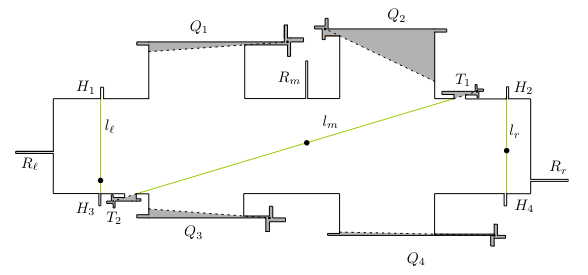
\includegraphics[width=0.7\textwidth]{Screenshot from 2022-01-21 12-46-51.png}
    \caption{Rectilinear Polygon $\mathcal P_R$}
    \label{fig:rectilinear}
\end{figure}
% a guard at position $x$ sees a point $y$ if the line segment $xy$ is fully contained in the polygon $\mathcal{P}$
% - a _guard set_ $S$ is a set of points in $\mathcal{P}$ s.t. every point in $\mathcal{P}$ is seen by some point in $S$ - find a minimum cardinality guard set for a simple polygon $\mathcal{P}$ on $n$ vertices
% - research less focussed on the classical problem, but more on its variations
% - no combinatorial algorithm for finding an optimal solution, or even for deciding whether a guard set of a given size $k$ exists, only real algebraic geometry powerful tools - not known if in NP
% - given polygons by integer coordinates, do they require guard positions with irrational coordinates in any optimal solution?
	% => yes, by constructing a _monotone_ polygon ($\exists$ line $l$ s.t. every line orthogonal to $l$ intersects $\mathcal P$ at most twice) with integer coordinates that can be guarded by three guards only when we allow to place the guards at points with irrational coordinates; otherwise, 4 guards are needed
			% - *place pic*
			% - **forcing a guard on a line segment** by creating 3 triangular pockets *pic* that can enforce 3 guards on 3 line segments within $\mathcal P$ - a guard can see both $t$ and $b$ if it is on the blue line segment $tb$, which is the intersection of 2 regions => $k$ pairs of triangular pockets and no 2 regions corresponding to different pairs of pockets intersecting => in order to guard the polygon with $k$ guards, there must be one guard on the line segment corresponding to each pair
			% - **restricting a guard to a region bounded by a curve** - consider a fixed position of $g_2$ on or to the right of the segment $bd$. $\exists$ a position of $g_1$ on $l$ s.t. the entire polygon is seen by $g_1$ and $g_2$ iff. $g_2$ lies on or to the left of the curve $\mathcal C$ *insert pic*
			% - **restricting a guard to a single (irrational) point** - *insert pic* $g_m$ and $g_l$ can guard together the 2 left pockets, and at the same time $g_m$ and $g_r$ can guard together the two right pockets => $g_m$ can only be in the irrational point $p = (3.5 + 5\sqrt 2, 1.5\sqrt 2)$
			% - **searching for the polygon** - we need to force $g_m$ to be on a line $l_m$ containing $p$, but we can only force $g_m$ to be on a rational line => we require the existence of a rational line $l_m$ that contains $p$ - there can be at most one rational line containing the irrational point $p$, as any 2 rational lines intersect in a rational point => reverse-engineer the polygon, after having chosen the positions of the guards of the form $(r_1 + r_2\sqrt 2, r_3 + r_4\sqrt 2), r_1, r_2, r_3, r_4 \in \mathbb Q$ ; rectangle with pockets added
	% - consider any set $S$ for $\mathcal P$ consisting of at most 3 guards: then $|S| = 3$ and $\exists$ 1 guard on each of the lines $l_l, l_m, l_r$
	% - consider any guard set $S$ for $\mathcal P$ consisting of 3 guards; then 1 of the guards has an $x$-coord in $[10.5, 10.6]$. For the remaining 2 guards, $g_l$ has a $y$-coord in $i_1 = [0.5, 0.6]$ and the $g_r$ in $i_2 = [1.7, 1.8]$
	% - **dependencies between guard positions**
		% - the guards $g_l$ and $g_m$ together see all of $e_t^l$ and $e_b^l$ and the guards $g_m$ and $g_r$ together can see all of $e_t^r$ and $e_b^r$ *add pic*
	% - **computing the unique solution**
		% - the max $x$-coord of $g_m$ s.t. $g_l$ and $g_m$ can together see $e_t^l$ and $e_b^l$ is $x = 3.5 + 5\sqrt 2$. The corresponding position of $g_l$ is $(2, 2 - \sqrt 2)$
		% - the min $x$-coord of $g_m$ s.t. $g_r$ and $g_m$ can see both $e_t^r$ and $e_b^r$ is $x = 3.5 + 5\sqrt 2$. The corresponding position of $g_r$ is $(19, 1 + \frac{\sqrt 2}{2})$  
	% - $\forall n$, there is a family of polygons $(\mathcal{P}_n)_{n \in \mathbb{Z}_+}$ which can be guarded by $3n$ guards with irrational coordinates, but need $4n$ guards to be rational; the coordinates of the points defining the polygons $\mathcal P_n$ are polynomial in $n$
	% - there is a rectilinear polygon $\mathcal P_R$ given by integer coordinates that require guards with irrational coordinates in any optimal solution - $\mathcal P_R$ can be guarded by 9 guards if we allow placing guards at points with irrational coordinates; an optimal guard set of $\mathcal P_R$ with guards at points with rational coordinates has size 10
		% - start with $\mathcal P$ - extend the non-rectilinear parts by "equivalent" rectilinear parts (gray) s.t. each of them requires at least  1 guard in the interior; if the interior of each pocket contains only 1 guard, then these guards must be placed at specific positions, making the area not seen by these 6 additional guards (white) => the remaining 3 guards must be placed at 3 irrational points (*place pic*)
% - _terrain guarding problem_ - $x$-monotone polygonal curve $c$ is given, the region $R$ above $c$ has to be guarded, and the guards are restricted to lie on $c$ - discretisation available in $O(n^3)$ time -> no irrational numbers phenomenon, and the decision version of the terrain guarding problem is in NP
\section{Theory}

\subsection{Computing the Gradient}

Let $\mathcal P$ be a polygon and $p(x, y) \in \mathcal P$ a guard. We are interested in computing the best direction for moving $p$ inside $\mathcal P$ such that the visibility area $Vis(p)$ increases. That is, exploring what would be a better position for $p$ such that $p$ ``sees more'' of the polygon $\mathcal P$. 

We can define $f(p)$ as the area seen by a guard $p$. Let $f'_i(p)$ be the local change in the area seen by guard $p$ around a reflex vertex $i$ of $\mathcal P$, as given by the derivative of $f$. Given all reflex vertices $i$, the total (global) change in the area seen by $p$ can be thus summed up to $f'(p) = \sum_i f'_i(p)$. Figure \ref{fig:sumf} offers an example for this case for a polygon $\mathcal P$ and its reflex vertices $r_1$ and $r_2$. The polygon $\mathcal P$ is guarded by $p$, and its position is modified to $p'$ by a small change $\partial y$. The visibility areas of $p$ become $f'_{r_1}$ and $f'_{r_2}$ around reflex vertices $r_1$ and $r_2$, respectively. In this way, the total change in the visibility area of $p$ becomes $f'(p) = f'_{r_1}(p) + f'_{r_2}(p)$.

Thus, $f(p)$ is the continuous objective function of The Art Gallery Problem. We can then use gradient descent as a method to optimise the objective function $f$. We will define below what the methodology of gradient descent is comprised of.

\begin{figure}[h!]
    \centering
    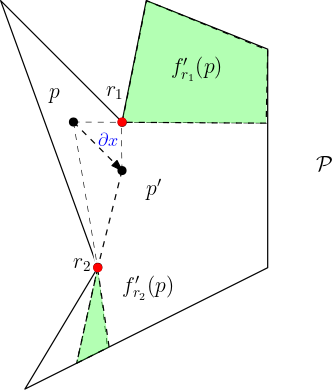
\includegraphics[width=0.4\textwidth]{sumf.png}
    \caption{Global change in the area seen by $p$ when moved by $\partial y$ to a new position $p'$.}
    \label{fig:sumf}
\end{figure}

Gradient descent is an iterative optimisation algorithm for finding the local maximum of a continuous differentiable function. The idea of gradient descent is to repeatedly move in the opposite direction of the gradient of the function at the current point. In this way, we can define $\bigtriangledown f$ to be the gradient of $f$. The gradient $\bigtriangledown f$ will then indicate the direction of the steepest descent for the objective function $f(p)$. 


% defining the gradient for computing the best change in the position of $p$.

Given that $f$ is a function that describes the visibility area of a point $p(x, y)$, we will first need to define how its gradient is computed. In order to simplify the gradient computation without losing generality, we will analyse the gradient by fixing one of the coordinates of $p$ and varying the other one. In this case, fixing the $x$-coordinate and varying the $y$-coordinate. As such, the computation of the gradient remains the same regardless of the rotation applied to the plane.


We will use the notation $\frac{\partial f}{\partial y}$ to denote the change in the visibility area $f(p)$ when the $y$-coordinate is modified by a small amount $\partial y \rightarrow 0$. Analogously, we will use $\frac{\partial f}{\partial x}$ to denote the small change in the $x$-coordinate of $p$. In this way, we define 

\begin{equation}
    \bigtriangledown f = (\frac{\partial f}{\partial x}, \frac{\partial f}{\partial y}) \label{eq:gradient}
\end{equation}

to be the gradient of $f$ given that $\mathcal P$ is guarded by a point $p(x, y)$. 

We will now create a canonical geometrical construction that will allow us to further define and compute $\bigtriangledown f$. In this case, we consider the normalised length of the gradient as $||\bigtriangledown f|| = 1$. This canonical construction is displayed in Figure \ref{fig:gradient}. We will then generalise this case to multiple reflex vertices and guards.

\begin{figure}[h!]
    \centering
    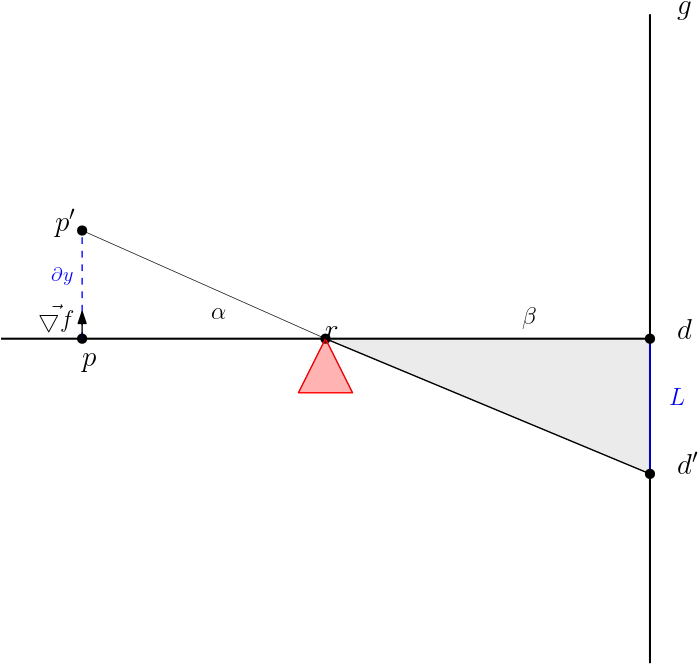
\includegraphics[width = 0.6\textwidth]{gradient2.png}
    \caption{Canonical gradient construction and for when the position of $p$ is varied by a small amount $\partial y$.}
    \label{fig:gradient}
\end{figure}

Let $g$ be a boundary line segment of $\mathcal P$, $r$ a reflex vertex inside $\mathcal P$ and $p$ a guard whose optimal position we are interested in. Let $\overline{pr} = \alpha$ be known. Additionally, let $d$ be the maximum point of visibility that $p$ can see behind $r$ on the line $g$. Let the distance between $r$ and $d$ be considered as $|\overline{rd}| = \beta$ known. 
% That is, the direction of the greatest increase of $f$. 

% We consider the case where there is only a positive change in the $y$ position of $p$. The case with a negative coordinate change would be analogous.


Let $\partial y$ be an extremely small change in the position of $p$. Call $p'$ this new position of $p$. The point $p'$ can see then up to a new maximum point $d'$ around $r$ on $g$. Let thus the distance between $d$ and $d'$ be $|\overline{dd'}| = L$. As such, $\triangle rdd'$ denotes the increase in the visibility area of $p$ when it moves to position $p'$. That is, the first derivative $f'(p)$ of $f$ will represent the change in the visibility area of $p$:

\begin{equation}
    \text{Area}_{\triangle rdd'} = f'_r(p). \label{eq:derivative}
\end{equation}

% Let $a''$ be the projection of $p'$ on $p''r$, and $a$ the projection of $a''$ on the line $pr$ such that the distance from $a$ to $r$ is $|\overline{ar}| = \alpha$. Take the distance between $p$ and $p'$ to be $x$. Since $a''$ is the projection of $p'$ on $pr$, then $|\overline{pp'}| = |\overline{aa''}| = x$.





% \subsection{Canonical Case}
% Consider the geometrical construction in Figure \ref{fig:gradient}. The construction was created for ease of computation, and the general case can be translated and rotated to this case.

% In this canonical case we will consider the situation where the gradient is normalised as $||\bigtriangledown f|| = 1$. 

We are now interested in computing how the area seen by guard $p$ increases given the change $\partial y$ in the position of $p$. The distances $||\overline{pr}|| = \alpha$ and $||\overline{rd}|| = \beta$ are known, so we aim at expressing the gradient $\bigtriangledown f$ through $\alpha$ and $\beta$. Since $\bigtriangledown f$ depends on the change in the coordinates of $p$, computing it is tightly connected to the change in the area of triangle $\triangle rdd'$. We will proceed to calculate the area of $\triangle rdd'$ below.
% We are now interested in computing the distances $|\overline{df}|, |\overline{aa'}|, |\overline{pp''}|, L$ such that we can compute the increase in the area seen by $p$ and thus the gradient $\bigtriangledown f$. The two triangle areas that need to be computed in order to do so are $A_{\triangle rdd'}$ and $A_{\triangle rdd''}$.

Given that triangles $\triangle rpp'$ and $\triangle rdd'$ are square triangles, their areas can be calculated as:

\begin{align}
    \text{Area}_{\triangle rpp'} &= \frac{\alpha \partial y}{2}, \label{eq:rpp}\\
    \text{Area}_{\triangle rdd'} &= \frac{\beta L}{2}. \label{eq:rdd}   
\end{align}


Given that $\overline{pp'}$ is parallel to $g$, we can use Thales's Theorem in triangles $\triangle rpp'$ and $\triangle rdd'$ to compute the length $L$: 

\begin{align}
    \frac{||\overline{pp'}||}{||\overline{dd'}||} &= \frac \alpha \beta \\
    \frac{\partial y}{L} &= \frac \alpha \beta  \label{eq:dxL} \\
    L &= \frac{\beta \partial y}{\alpha}. \label{eq:L}
\end{align}


% we can compute the length $L$: $$\frac{\text{Area}_{\triangle rdd'}}{\text{Area}_{\triangle rpp'}} = \frac{\frac{\beta L}{2}}{\frac{\alpha \partial x}{2}} = \frac{\beta L}{\alpha \partial x} \Rightarrow L = \frac{\partial x \beta}{\alpha}.$$

We are now interested in how areas $\text{Area}_{\triangle rpp'}$ and $\text{Area}_{\triangle rdd'}$ change depending on how $\alpha$ and $\beta$. That is, $\frac{\text{Area}_{\triangle rdd'}}{\text{Area}_{\triangle rpp'}}$ as a function of $\alpha$ and $\beta$: 

\begin{align}
    \frac{\text{Area}_{\triangle rpp'}}{\text{Area}_{\triangle rdd'}} \overset{(\ref{eq:rpp}), (\ref{eq:rdd})}{=} &\frac{\frac{\alpha \partial y}{2}}{\frac{\beta L}{2}} \\
    = &\frac{\alpha \partial y}{\beta L} \\
    \overset{(\ref{eq:dxL})}{=} &\frac{\alpha \alpha}{\beta \beta} \\
    \frac{\text{Area}_{\triangle rpp'}}{\text{Area}_{\triangle rdd'}} = &{(\frac \alpha \beta)}^2 \label{eq:rddrpp}
\end{align}

We can now express the area of $\triangle rdd'$ as only dependent on $\alpha, \beta$, the small position change $\partial y$ and the already known area of $\triangle rpp'$:

\begin{align}
    \text{Area}_{\triangle rdd'} \overset{(\ref{eq:rddrpp})}{=} &{(\frac \beta \alpha)}^2 \text{Area}_{\triangle rpp'} \\
    \overset{(\ref{eq:rpp})}{=} &{(\frac \beta \alpha)}^2 \frac{\alpha \partial y}{2} \\
    \text{Area}_{\triangle rdd'} = &\frac{\beta^2 \partial y}{2\alpha}. \label{eq:ardd}
\end{align}
% \end{align*}
% $$\frac{\partial f}{\partial x} = \frac{\text{Area}_{\triangle rdd'}}{\partial x}$$

Analogously, we can compute the change in the $y$-coordinate by rotating the plane with $90^\circ$ and follow the same steps. This procedure will result in

\begin{equation}
    \text{Area}_{\triangle rdd'} = \frac{\beta^2 \partial y}{2\alpha}. \label{eq:ardd2}
\end{equation}

We can now compute the change in the visibility area $\text{Area}_{\triangle rdd'}$ of $p$ given the movement $\partial y$ in the position of $p$. Since the $x$-coordinate of $p$ is fixed, so $\partial x = 0$, the gradient $\bigtriangledown f$ is 

\begin{align*}
    \bigtriangledown f \overset{(\ref{eq:gradient})}{=} &(\frac{\partial f}{\partial x}, \frac{\partial f}{\partial y}) \\
    \overset{(\ref{eq:derivative})}{=} &(0, \frac{\text{Area}_{\triangle rdd'}}{\partial y} + \partial y) \\
    \bigtriangledown f \overset{(\ref{eq:ardd}), (\ref{eq:ardd2})}{=} &(0, \frac{\beta^2}{2\alpha} + 0) \\
    \bigtriangledown f = &(0, \frac{\beta^2}{2\alpha}).
\end{align*}

Analogously, when $p$ is moved along the $x$-axis with a fixed $y$-coordinate, the gradient becomes $$\bigtriangledown f = (\frac{\beta^2}{2\alpha}, 0).$$

\subsection{Computing the New Guard Position}

We can now compute the optimised position of the guard, given the computation of the gradient. In order to do so, we will use the construction depicted in Figure \ref{fig:vperp}. 

\begin{figure}[h!]
    \centering
    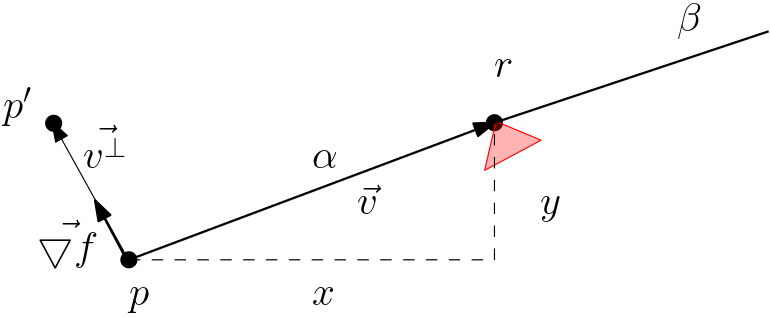
\includegraphics[width = 0.5\textwidth]{v_perp.png}
    \caption{Computing the new position $p'$ of guard $p$ around reflex vertex $r$ based on the gradient $\bigtriangledown f$.}
    \label{fig:vperp}
\end{figure}

Let vector $\vec{v} = (r - p) = (x, y)^\intercal$, with norm $||v|| = \alpha$. So, $||\frac{\vec v}{\alpha}|| = 1$.

Let vector $\vec{v}^\perp$ be the orthogonally translated vector to $\vec{v}$, in the same direction as $\vec{\bigtriangledown f}$, such that $||\vec{v}|| = ||\vec{v}^\perp|| = \alpha$.

The coordinates of $\vec v^\perp$ can then be computed using the construction from Figure \ref{fig:vsquare}. Since $\vec v^\perp \perp \vec v$, and $p$ and $r$ are on the right-hand side of $\vec v^\perp$, the coordinates of $\vec v^\perp$ will be rotated by $-90^\circ$ so that $\vec v^\perp = (-y, x)^\intercal$. Analogously for the case when $p$ and $r$ are rotated by $180^\circ$ to the left-hand side of $\vec v^\perp$, the coordinates of $\vec v^\perp$ will be rotated by $90^\circ$ to $\vec v^\perp = (-x, y)^\intercal$.

\begin{figure}[h!]
    \centering
    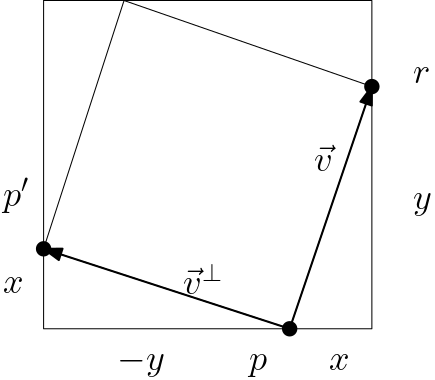
\includegraphics[width = 0.5\textwidth]{v_square.png}
    \caption{Computing the coordinates of $\vec v^\perp$ given the guard $p$ and the reflex vertex $r(x, y)$.}
    \label{fig:vsquare}
\end{figure}

We know that the norm of the gradient is $||\vec{\bigtriangledown f}|| = \frac{\beta^2}{2\alpha}$. Since $\vec{\bigtriangledown f}$ has the same direction as $\vec v^\perp$ and we wish to normalise it from the norm of $\vec v^\perp$ with $\frac 1 \alpha$, the gradient can be computed as $$\vec{\bigtriangledown f} = \vec v^\perp \frac{\beta^2}{2\alpha} \frac 1 \alpha.$$





% Given that $pp''$ is parallel to $g$, we can use the Intercept Theorem to compute the lengths of the segments as follows:

% \begin{itemize}
%     \item in $\triangle raa'$, $\triangle rpp'$, with $aa' || pp'$: $$\frac{|\overline{pp'}|}{|\overline{dd'}|} = \frac{|\overline{pr}|}{|\overline{rd}|} \iff \frac{x}{|\overline{dd'}|} = \frac{1}{\beta} \Rightarrow |\overline{dd'}| = x\beta$$
    
%     $$\frac{|\overline{aa'}|}{|\overline{pp'}|} = \frac{\alpha}{1} = \frac{|\overline{aa'}|}{x} \Rightarrow |\overline{aa'}| = x\alpha$$

%     \item in $\triangle rpp''$, $\triangle raa''$, with $pp'' || aa''$: $$\frac{|\overline{aa''}|}{pp''} = \frac{|\overline{ar}|}{|\overline{pr}|} \iff \frac{x}{|\overline{pp''}|} = \frac{\alpha}{1} \Rightarrow |\overline{pp''}| = \frac{x}{\alpha}$$
    
%     \item in $\triangle rpp''$, $\triangle rdd''$, with $pp'' || dd''$: $$\frac{|\overline{pp''}|}{|\overline{dd''}|} = \frac{|\overline{pr}|}{|\overline{rd}|} \iff \frac{\frac{x}{\alpha}}{L} = \frac{1}{\beta} \Rightarrow L = \frac{x\beta}{\alpha}$$
% \end{itemize}

% Now the area of the square triangle $\triangle rdd''$ corresponding to the gradient $\bigtriangledown f$ can be computed as: $$\bigtriangledown f = \frac{|\overline{rd}||\overline{de}|}{2} = \frac{\beta L}{2} = \frac{\beta \frac{x\beta}{\alpha}}{2} = \frac{\beta^2x}{2\alpha}, ||x|| = 1$$


% \subsection{General Case}


% - we will only look at one coordinate (vary $y$), since varying $x$ is symmetrical, but rotated $90^\circ$

% - we will first look at a canonical situation $||\bigtriangledown f|| = 1, \alpha = \beta = 1$

% Let:

% - $f(p)$ - area seen by guard $p$

% - $f'_i(p)$ - the change in the area seen locally by guard $p$, as given by its derivative

% - $f'(p) = \sum_i f'_i(p)$ - the change in the area seen globally by guard $p$

% - $\bigtriangledown f = (\frac{\partial f}{\partial x}, \frac{\partial f}{\partial y})$ - the direction of the greatest increase of $f$

% - $r$ - reflex vertex

% - $p$ - guard whose position needs to be optimised

% - $|\overline{pr}| = 1$

% - $p', p''$ - the new positions of the guard where the $y$-coord is varied

    % - $|\overline{pp'}| = |\overline{aa''}| = x$

% - $\overline{ar} = \alpha, a \in \overline{pr}$ - additional guard construction

% - $\triangle rde$ - area seen by $p$

    % - $\triangle rdf$ - area seen by $p'$

% - $|\overline{rd}| = \beta$ - distance between reflex vertex and polygon boundary

% - $|\overline{de}| = L$

% Using the Intercept Theorem:

% - in $\triangle ra'a$, $\triangle rp'p$: $\frac{|\overline{pp'}|}{|\overline{df}|} = \frac{|\overline{pr}|}{|\overline{rd}|} = \frac{x}{|\overline{df}|} = \frac{1}{\beta} \Rightarrow |\overline{df}| = x\beta$

% - in $\triangle pp'r$, $\triangle aa'r$: $\frac{|\overline{aa'}|}{|\overline{pp'}|} = \frac{\alpha}{1} = \frac{|\overline{aa'}|}{x} \Rightarrow |\overline{aa'}| = x\alpha$

% - in $\triangle pp''r$, $\triangle aa''r$: $\frac{|\overline{aa''}|}{pp''} = \frac{|\overline{ar}|}{|\overline{pr}|} = \frac{x}{|\overline{pp''}|} = \frac{\alpha}{1} \Rightarrow |\overline{pp''}| = \frac{x}{\alpha}$

% - in $\triangle pp''r$, $\triangle rde$: $\frac{|\overline{pp''}|}{|\overline{de}|} = \frac{|\overline{pr}|}{|\overline{rd}|} = \frac{\frac{x}{\alpha}}{L} = \frac{1}{\beta} \Rightarrow L = \frac{x\beta}{\alpha}$

% Computing the area of the square triangle $\triangle rde$:

% - $A = \frac{|\overline{rd}||\overline{de}|}{2} = \frac{\beta L}{2} = \frac{\beta \frac{x\beta}{\alpha}}{2} = \frac{\beta^2x}{2\alpha}$
% \section{Theory and Literature}



\subsection{Reinforcement Learning}
Machine learning is concerned with algorithms that learn from experience over time by processing information. Reinforcement learning is the branch of AI and machine learning where an intelligent agent tries to maximize its total reward by performing actions in an environment. In other words, an agent interacts with its environment and learns to adjust the environment towards preferred states. 

\begin{figure}[h]
    \centering
    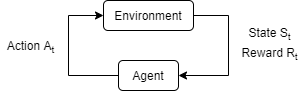
\includegraphics[width = 8cm]{Figures/RL Diagram.png}
    \caption{\centering Agent-environment interaction in reinforcement learning.}
    \label{fig: RL diagram}
\end{figure}
\noindent
An agent may like or dislike the current state of its environment. This preference is represented by a reward signal. The agent goes through a repeating sequence of states, rewards, and actions (figure \ref{fig: RL diagram}). Such a sequence from beginning to end is called a trajectory. The goal of the agent is to take actions that result in a trajectory with the highest total reward. The total reward of an entire trajectory is called the return. 


The agent chooses what actions to take based on its current state. The action strategy is called the policy '$\pi$'. The policy of an agent determines the action probability from any state. An action $A_t$ is drawn from the policy $\pi(A_t|S_t)$ of the agent. Similarly a state $S_t$ is drawn from the state-transition probability distribution $P(S_{t+1}|S_t,A_t)$ of the environment. The difference is that the state-transition dynamics do not change, while the policy is updated in an attempt to maximize the agent's return.





\subsubsection*{The Return}
The agent receives an observation of the state $S_t$ and a reward signal $R_t$ at time \textit{t}. The return is generally determined as the discounted sum of rewards in a trajectory:

\begin{equation}
    G_t = \sum_{k=t+1}^{T} \gamma^{k-(t+1)} R_k,
    \label{eq: return}
\end{equation}

\noindent
where successive returns are related to each other by:

\begin{equation}
    G_t = R_{t+1} + \gamma G_{t+1}.    
    \label{eq: return sequence}
\end{equation}
\\[-3mm]
\noindent
Equation \ref{eq: return} defines the \textit{return} as the summation over rewards multiplied by the discount factor $\gamma \in (0,1)$ from the start until termination time T. The discount factor is included to penalize distant rewards. There is no penalty when $\gamma = 1$, and only the first reward has value to the agent when $\gamma = 0$. The optimal discount factor depends on the problem, but is usually $\sim$0.99. 




\subsubsection{Value Functions}
Each state has a \textit{value} that determines how much reward the agent is expected to get from that particular state onward. It is useful to know these state values, since agents can then take actions that direct them towards higher valued states. The value of a state is defined as the expected return of that state:

\begin{equation}
    \label{eq: state value function}
    V^\pi(s) = \mathbb{E}_\pi[G_t\ |S_t = s].
\end{equation}
\\[-3mm]
\noindent
This is the \textit{state-value function} following policy $\pi$. The value of state 's' is equal to its estimated return. Another useful value function is the action-value function. This function estimates the value of a state-action pair:

\begin{equation}
    Q^\pi(s,a) = \mathbb{E}_\pi[G_t\ |S_t = s, A_t = a].
    \label{eq: action value function}
\end{equation}
\\[-3mm]
\noindent
The \textit{action-value function} following policy $\pi$ describes the expected return if the agent starts in state s, performs action a, and from there takes actions based on policy $\pi$ until termination. 
\\\\
The advantage of an action is a measure of how good the action is in a particular state. Th \textit{advantage function} can be calculated by subtracting equation \ref{eq: action value function} from equation \ref{eq: state value function} for a specific action: 
\\[-3mm]
\begin{equation}
    A^\pi(s,a) = Q^\pi(s,a) - V^\pi(s).
\end{equation}
\\[-2mm]
\noindent
The advantage function can be seen as the Q-function with lower variance since the V-value is subtracted as a baseline. If the advantage function is positive for a state-action pair, the agent expects more return in state s from performing action a than following policy $\pi$.

\subsubsection*{Optimal Policy}

If the value function following policy $\pi$ is at its maximum for all states, this policy is called optimal. There is always at least one optimal policy $\pi^*$.  If the state-value and action-value functions follow the optimal policy, these functions are by definition also optimal:
\\[-4mm]
\begin{gather}
        \label{eq: V optimal}
        V^*(s) =  \underset{\pi}{max} \, V^\pi(s), \\ 
        Q^*(s,a) =  \underset{\pi}{max} \, Q^\pi(s, a).
        \label{eq: Q optimal}
\end{gather}
\\[-2mm]
\noindent
Function \ref{eq: V optimal}  and \ref{eq: Q optimal} are the \textit{optimal state-value function} and the \textit{optimal action-value function}. These functions follow the policy that returns the highest value for each state. The optimal policy is only known in very simple problems like tic-tac-toe. In more difficult environments like chess, it becomes infeasible to find the optimal policy due to the enormous number of possible trajectories. Finding a policy as close to this optimal policy as possible is at the heart of reinforcement learning. 

\newpage

\subsubsection*{The Bellman Equations}

Approaching the real values of the value functions is an optimization problem. The Bellman equations are equations that break down this optimization problem into multiple simpler problems. There are four Bellman equations. The first Bellman equation states that the current value of a state is the reward from that state plus the value of the next state:

\begin{equation}
    \label{eq: 1st bellman equation v-policy}
    V^\pi(s) =  \underset{\underset{s' \sim P}{a' \sim \pi }}{\mathbb{E}} \ [R(s,a')\ +\ \gamma V^\pi(s')].
\end{equation}
\\
\noindent
Here, the a' and s' stand for the upcoming action and state drawn from the policy and the environment. The reward plus next value on the right side of the equation is called the \textit{Bellman backup}.

As for the state's V-value, there is also a Bellman equation for the state-action Q-value. Similar to the previous equation \ref{eq: 1st bellman equation v-policy}, this Bellman equation finds its value by the current reward plus the value of the next state-action pair:

\begin{equation}
    \label{eq: 2st bellman equation q-policy}
    Q^\pi(s,a) =  \underset{\underset{s' \sim P}{a' \sim \pi }}{\mathbb{E}} \ [R(s,a)\ +\ \gamma Q^\pi(s',a')]
\end{equation}


\begin{equation*}
    = \underset{a}{\sum}  \pi(a|s) \underset{s'}{\sum} P(s'|s,a) \ 
    [R(s,a)\ +\ \gamma Q^\pi(s',a')].
\end{equation*}
\\
\noindent
This equation is expanded to find the meaning of the expectation $\mathbb{E}$. The expectation averages all possibilities weighted by the probability of occurring. In the case of equation \ref{eq: 2st bellman equation q-policy}, the Q-value is estimated as a weighed sum over the possible actions and states multiplied by the Bellman backup. These actions a' and states s' are given by the policy and the state-transition distributions. Both these distributions sum up to one, since each time-step includes one action and one state.

The final two Bellman equations are the optimal versions of equation \ref{eq: 1st bellman equation v-policy} and \ref{eq: 2st bellman equation q-policy}. They are similar to the previous equations, except for the choice of the upcoming action a'. Instead of summing over each possible action in the policy, an optimal action is selected.



\begin{gather}
    \label{eq: 3rd bellman equation v-optimal}
    V^*(s) = \underset{a'}{max} \underset{s' \sim P}{\mathbb{E}} \ [R(s,a')\ +\ \gamma V^*(s')], \\ 
    Q^*(s,a) =  \underset{s' \sim P}{\mathbb{E}} \ [R(s,a)\ +\ \gamma \, \underset{a'}{max} \, Q^*(s',a')].
    \label{eq: 4rd bellman equation q-optimal}
\end{gather}
\\[-2mm]
\noindent
In these optimal Bellman equations, the action a' is chosen such that the return is maximized. In a solved optimization problem, the V*-values and Q*-values are the true state and action values. In this case, an optimal policy always takes an action that obeys:

\begin{equation}
    A^* = arg\, \underset{a}{max} \, Q^*(s,a).
\end{equation}


\newpage












\subsubsection{Learning from Interaction}

In reinforcement learning, there are two main methods to learn the state and action value functions from interaction with an environment. These are the Monte Carlo and Temporal Difference methods. 

\subsubsection*{Monte Carlo}

\textit{Monte Carlo} (MC) is a class of learning methods where the values are updated only after an entire episode is generated. Each episode is a trajectory of state-action-reward time-step from start to finish. This trajectory is sampled from the probability distributions of the environment's dynamics and the agent's policy. After an episode is generated, the return at each time-step t in this episode is calculated from the final step backwards. Each value is updated by:

\begin{equation}
    \label{eq: Monte Carlo Value Update}
    V(S_t) \leftarrow V(S_t) + \alpha [G_t - V(S_t)].
\end{equation}
\\[-2mm] \noindent
The syntax of this update on the state value function $V(S_t)$ also works to update the action value function $Q(S,A)$. In the update the $[G_t - V(S_t)]$ term represents the difference between the sampled return G and the expected return V at time t. The return G is called the \textit{target}, and the value V is updated to better resemble this target. $\alpha \in (0,1)$ is the step size that determines the rate of learning. Nothing new will be learned when $\alpha = 0 $, and only the newest sample is taken into account when $\alpha = 1$. In practice, an $\alpha$ of $\approx 0.00025$ balances between these two extremes. 




\subsubsection*{Temporal Difference}

As with Monte Carlo, \textit{temporal difference} (TD) methods learn from experience without a model of the environment's dynamics. The main difference between the two methods is that temporal difference methods \textit{bootstrap}. With bootstrapping the value estimates are updated with the use of other value estimates. This makes it possible to update the value function without the need to finish an entire episode:

\begin{equation}
    V(S_t) \leftarrow V(S_t) + \alpha [(R_{t+1} + \gamma V(S_{t+1})) - V(S_t)].
\end{equation}
\\[-2mm] \noindent
The value of a state is updated by only using the next reward $R_{t+1}$ and next state value $V(S_{t+1})$. The values can thus be updated directly after each step. The target $(R_{t+1} + \gamma V(S_{t+1}))$ is motivated by the Bellman backup of equation \ref{eq: 1st bellman equation v-policy}. The value is updated a step $\alpha$ in the direction of this target. 

A Monte Carlo trajectory produces an unbiased estimation of the value of each visited state, since the actual return is used as a target. However, due to the broad range of possible trajectories the variance of the return is high. In contrast, temporal difference include a bias, since the values are based on other value estimations and not solely on observations. However, bootstrapping has a lower variance as an advantage. 

The two main TD methods are Sarsa and Q-learning. The difference between these two methods is that Sarsa learns on-policy, and Q-learning learns off-policy. An explanation on this difference is given after the reinforcement learning problem is explained. % (\ref{eq: SARSA update} and \ref{eq: Q-learning update}).


\subsubsection*{Prediction and Control}

% Prediction
The reinforcement learning problem can be split into a prediction and a control problem. In the \textit{prediction problem} the state values are estimated based on the current policy. In the \textit{control problem} the policy is updated to better suit the latest estimated values. The value and policy are repeatedly updated in succession with respect to each other. In theory, this iterative interaction of prediction and control converges to a global optimum. However, in practice the process does not always converge or gets stuck in a local optimum. This instability can have multiple reasons like insufficient data, improper hyperparameters, or a learning method that is unfit for the problem. Moreover, the agent needs to properly balance exploration with exploitation to approach a global optimum. 

\subsubsection*{Exploration and Exploitation}

With \textit{exploitation} the agent chooses actions that are expected to return the highest reward. Exploitation is needed to increase data on the most promising states and actions. By only exploiting, trajectories that initially show little return are not further explored. This makes it possible to get trapped in a local optimum. The policy of an agent should therefore also include \textit{exploration}. For example, the $\epsilon$-greedy policy chooses an action at random with probability $\epsilon$, and otherwise acts to maximize expected return.

\subsubsection*{On-Policy and Off-Policy}
The value function can be learned on-policy and off-policy. Both these learning methods balance exploration with exploitation differently. With \textit{on-policy} learning, the actions are sampled from the same policy that is optimized. With \textit{off-policy} learning, the learned behavior does not necessarily reflect the agent's actions. Off-policy methods use two separate policies, the target policy and the behavior policy. The goal in off-policy learning is to optimize for the \textit{target policy} while taking actions from the \textit{behavior policy}. Due to this separation between the two policies, off-policy methods are more general. Off-policy learning enables \textit{experience replay} where an agent learns by reviewing stored experiences. These stored experiences do not have to be from the learning agent itself.




\subsubsection*{Sarsa}
\textit{Sarsa} is the most basic on-policy, temporal difference, control method. Because Sarsa is a control method the action value function $Q(S,A)$ is used instead of the state value function $V(S,A)$: 

\begin{equation}     \label{eq: SARSA update}
    Q(S_t, A_t) \leftarrow Q(S_t, A_t) + \alpha [(R_{t+1} + \gamma Q(S_{t+1}, A_{t+1}))  - Q(S_t, A_t) ].
\end{equation}
\\[-2mm] \noindent
The next action $A_{t+1}$ is sampled from the policy. This makes the action value update  on-policy. For example, an $\epsilon$-greedy policy chooses the action $A_{t+1}$ to maximize the value $Q(S_{t+1}, A_{t+1})$ with chance ($ 1-\epsilon$), or at random with chance $\epsilon$.

The next value $Q(S_{t+1}, A_{t+1})$ can itself be split up into into an upcoming reward and discounted value $R_{t+2} + \gamma Q(S_{t+2}, A_{t+2})$ to get a nested update of the action value. This technique of nested updates is called \textit{n-step bootstrapping}, where the temporal difference extends over the amount of nested steps n. If the steps are updated all the way through the end of the sample trajectory, the TD method becomes a Monte Carlo method.  










\subsubsection*{Q-Learning}

As with Sarsa, \textit{Q-learning} is a temporal difference, control method. The difference is that Q-learning is off-policy.  The target in the Sarsa update contains the action value $Q(S_{t+1}, A_{t+1})$ where the action that determines this action value is chosen by the policy. In contrast, the action in the target of Q-learning is chosen to maximize the action value:

\begin{equation}    \label{eq: Q-Learning update}
    Q(S_t, A_t) \leftarrow Q(S_t, A_t) + \alpha [(R_{t+1} + \gamma \, \underset{a}{max} \, Q(S_{t+1}, a))  - Q(S_t, A_t) ].
\end{equation}
\\[-2mm] \noindent
In this update the action \textit{a} that maximizes the value $Q(S_{t+1}, a)) $ is chosen to bootstrap the action value from. The behavior policy does not have an effect on this update, since the update always chooses the optimal action value regardless of the policy. This makes Q-learning off-policy.



% \subsubsection{Planning with Models}

% Some reinforcement learning methods improve solely from experience on the actual environment. These are called \textit{model-free} methods. Other methods require a model of the environment to operate, either to learn or to plan ahead. These are called \textit{model-based} methods. 

% planning versus learning, model

% Given vs learned model

% planning at decision time (MCTS)

% dynamic programming










\subsubsection{Neural Networks}

% 1. Why function approximation

In basic \textit{tabular methods} each value is stored individually. In many reinforcement learning problems however, the number of possible states of an environment vastly exceeds the number of computer bits. It is impossible to keep track of every value individually, due to the memory needed to store these values, and the time to get samples from each state. Luckily, the values can be approximated by generalizing between similar states. This generalizing is often done with the use of \textit{Artificial Neural Networks} (ANNs). An ANN takes for example a state as input and can generalize this state to similar observed states as a way to estimate the state's value. These networks are inspired by the structure of neurons inside a biological brain.

\subsubsection*{Feedforward Neural Networks}

An Artificial Neural Networks is a \textit{non-linear function approximator}. ANNs can approximate any function depending on the structure of the ANN. An ANN is made up of multiple \textit{nodes} that are connected with \textit{edges}. A \textit{feedforward neural network} is a network where the nodes in each layer are connected to nodes in the next layer. The first and last layers are the input and output layers, and the layers in the middle are the \textit{hidden layers}. 


With \textit{fully connected} (dense) layers, each node is connected to every node in the previous layer. According to the universal approximation theorem, one hidden dense layer with an arbitrary number of nodes is enough to approximate any function.


%Another type of widely used NN is the convolutional neural networks (CNN). This class of NN is able to analyze images by looking at several levels of abstraction, by means of convolution and subsampling. 





\subsubsection*{Neurons}

Each node in a neural network acts as a simple individual function through which signals are passed:

\begin{equation}
    y_m = f( \underset{n}{\sum} \theta_{mn} x_n )
\end{equation}
\\[-2mm] \noindent
In this function, the node \textit{m} receives the output of other nodes $x_n$ as input. The input values are multiplied by the \textit{weights} $\theta_{mn}$ of the edges that connect each input node to node m. The weighted value of each input node is summed together. This resulting summation is inserted in the function \textit{f} to produce the output $y_m$ of node \textit{m}. 

The function \textit{f} is the \textit{activation function}. This function is required to add a non-linearity into the system. The non-linearity is needed because linear functions of linear functions are also linear, which would make them unfit to approximate non-linear function. A simple example of an activation function is the rectified linear unit (ReLU): $f(x) = max(0,x)$. Other popular activation functions are the S-shaped logistic function $f(x) = 1/(1+e^{-x})$ and the hyperbolic tangent function $f(x) = tanh(x)$. 









\subsubsection*{Backpropagation}

% 4. Loss + Backpropagation 

Feedforward neural networks can be trained with the \textit{backpropagation} algorithm. With backpropagation, the weights of the neural networks are updated via \textit{stochastic gradient descent} (SGD). Gradient descent is the principle where weights are adjusted in the direction of a lower error by taking the derivative of the loss with respect to each weight. The gradient descent is called stochastic when the training data is randomly sampled. 

The loss function \textit{L} is often calculated as the squared difference between the target Y and the estimated value of the ANN:

\begin{equation}
    L(\WeightVector) = (Y - V(s;\WeightVector))^2
\end{equation}
$\WeightVector$ is the \textit{weight vector} that consists of all the weights in the ANN. Each weight can be individually adjusted to reduce the loss. This is done by taking a step $\alpha$ in the direction of steepest descent:

\begin{equation} \label{eq: individual weight update}
    \theta_{mn} = \theta_{mn} - \alpha \frac{\delta L}{\delta \theta_{mn}}
\end{equation}
This function can also be written for all weights simultaneously:


\begin{equation}
    \WeightVector = \WeightVector  - \alpha \nabla_{\theta} L
\end{equation}
The del operator $\nabla$ denotes the gradient operation. $-\nabla_{\theta} L$ points in the direction of steepest descent. The magnitude of $\nabla_{\theta} L$ is equal to the steepness of this slope. As the weight vector $\WeightVector$ is constantly updated in the direction of lower loss, the value estimations of the ANN get closer to the targets.


% Variable step size SGD: RMSProp/Adam etc

% mini-batch






% \subsubsection{Policy Gradient Methods}

% basics
% Neural network maps states to actions in the case of policy approximation.

% Policy Gradient Theorem

% REINFORCE or VPG, Monte-Carlo PG   baseline

% Actor Critic





% 


\newpage
\subsection{Deep Q-Learning}


\subsubsection{DQN Algorithm}

% Intro


The paper "Playing Atari with Deep Reinforcement Learning" \cite{Atari_DQN_2013} from Mnih et al. in 2013 revolutionized reinforcement learning in video games. In this paper, an agent surpasses humans on the Atari console from 1977 on multiple games by performing actions while observing the video images of the game. The same raw input, network architecture, and parameter values are used in each of the 49 Atari games. By learning a different policy for each game the agent learns to play at or beyond the skill level of humans on many of these games. The paper used its own \textit{Deep Q-Learning} (DQN) algorithm to achieve this.


% Deep Convolutional ANN / Preprocessed sequences / Experience replay

The DQN agent contains a \textit{deep convolutional} ANN. This is a multi-layered ANN that is specialized for processing spatial data arrays such as images. The raw images collected from the screen are seen as the state $s$ of the environment $\epsilon$. These states are pre-processed into $\phi(s)$ to reduce the input size for the Q-function.

DQN makes use of \textit{experience replay}. While playing the game, the agent stores transitions ($\phi_t, a_t, r_t, \phi_{t+1}$) in a \textit{replay memory} $\mathcal{D}$. During learning, these transitions are randomly sampled. 

% Equations

The loss is calculated as the square difference between the target $y_i$ and the action value function $Q(s,a;\theta_i)$:

\begin{equation}
    L_i(\theta_i) = \underset{s,a \sim  \rho(\cdot)}{\mathbb{E}} [(y_i - Q(s,a;\theta_i))^2]
\end{equation}

Here, $L_i$ is the loss at iteration \textit{i}, and $\rho(s,a)$ is the behavior distribution. The following gradient is obtained by differentiating the loss function with respect to the weights $\theta$:

\begin{equation}
    \label{eq: loss gradient DQN}
    \nabla_{\theta_i} L_i (\theta_i) = \underset{\underset{s' \sim  \varepsilon}{s,a \sim  \rho(\cdot)}}{\mathbb{E}} [(r + \gamma \, \underset{a'}{max} \, Q(s',a';\theta_{i-1}) - Q(s,a;\theta_i)) \nabla_{\theta_i}Q(s,a;\theta_i)]
\end{equation}






\noindent
The entire DQN algorithm is given below: 

\begin{algorithm}[H]
\caption{Deep Q-learning with Experience Replay \cite{Atari_DQN_2013}} \label{alg: Deep Q-learning}
\hspace*{2mm} Initialize replay memory $\mathcal{D}$ to capacity N \\
\hspace*{2mm} Initialize action-value function Q with random weights \\
\hspace*{2mm} \textbf{for} episode = 1, M \textbf{do} \\
\hspace*{7mm} Initialise sequence $s_1$ = $\{x_1\}$ and preprocessed sequenced $\phi_1 = \phi(s_1)$ \\
\hspace*{7mm} \textbf{for} t = 1, T \textbf{do} \\
\hspace*{12mm} With probability $\epsilon$ select a random action $a_t$ \\
\hspace*{12mm} otherwise select $a_t = max_a \, Q^*(\phi(s_t), a; \theta)$ \\
\hspace*{12mm} Execute action $a_t$ in emulator and observe reward $r_t$ and image $x_{t+1}$ \\
\hspace*{12mm} Set $s_{t+1} = s_t, a_t, x_{t+1}$ and preprocess $\phi_{t+1} = \phi(s_{t+1})$ \\
\hspace*{12mm} Store transition ($\phi_t, a_t, r_t, \phi_{t+1}$) in $\mathcal{D}$  \\
\hspace*{12mm} Sample random minibatch of transitions ($\phi_j , a_j , r_j , \phi_{j+1} $) from $\mathcal{D}$  \\
\hspace*{12mm} Set $y_j =  \begin{cases} r_j $ \hspace*{40mm}  for terminal $ \phi_{j+1}  \\ 
r_j + \gamma \, max_{a'} \, Q(\phi_{j+1}, a';\theta) $ \hspace*{2.5mm}  for non-terminal $ \phi_{j+1}  \end{cases}$ \\
\hspace*{12mm} Perform a gradient descent step on $(y_j - Q(\phi_j , a_j ; \theta))^2$ according to equation \ref{eq: loss gradient DQN} \\
\hspace*{7mm} \textbf{end for} \\
\hspace*{2mm} \textbf{end for}
\end{algorithm}











% \subsubsection{DQN Improvements}

% Rainbow 









%\subsection{Policy Optimization}





% \section{Thesis Project}


The main goal of this thesis is to create a superhuman artificial agent in \href{https://Slither.io}{Slither.io}. The agent is trained inside a replicated environment of the game, and will be deployed onto the game to test itself against real players. Additionally, the performance and computing efficiency of different machine learning methods are assessed.
\\



\subsection{Why Slither?} % 4.1
To me, it seems interesting to apply machine learning to Slither. In part because the player's situation can get complex quickly. The optimal playstyle depends on the behavior of the opponent snakes. The player needs to anticipate the moves of multiple snakes. Crucial information can present itself on screen at every time-step. This can make it hard to find a good move and work out a solid plan. The performance of an agent depends on clever anticipation and dexterous movement. It will be interesting to study how the differently trained agents will handle these complex situations. The agents will hopefully be able to reason in a way that humans consider intelligent. 
\\[2.5mm]
Even though the states are often complex, the game has only few controls. The only control options are the left, right, or forward direction, and an optional speed boost. This makes it less convoluted to the AI to deduce which action causes which environment change, compared to video games with multiple buttons, trigger and joysticks. Fewer controls are better for efficient training and lower computing costs.
\\[2.5mm]
Games can have multiple possible team formation configuration. The most common are 1-vs-1 as in chess, team-vs-team as in football, or playing against the game, as in consoles like Atari. In free-for-all games like poker every player competes against each other under the same circumstances. To my knowledge, reinforcement learning is not often applied to free-for-all video games with hundreds of players in a single arena like in Slither. 
\\






\subsection{Previous Attempts}  % 4.2

There have been two notable papers where agents learn to play Slither with deep reinforcement learning. Both papers make use of deep Q-Learning, as used in the famous Atari DQN paper \cite{Atari_DQN_2013}. One of these papers, "Learning to play SLITHER.IO with deep reinforcement learning" \cite{prev:Slither_2019} includes a replay buffer and human demonstrations for pre-training on top of DQN learning. Both replay learning and imitation learning greatly improve performance. The paper concludes with an acknowledgement that the more advanced actor-critic methods may result in better performance.
\\[2.5mm]
The other paper, "Slither.io Deep Learning Bot" \cite{prev:Slihter_2017_OpenCV} is written less formally, but contains an interesting idea. This paper uses the computer vision library OpenCV to transform the standard game view into a feature image. This feature image labels objects like the player's snake, other snakes, pellets, and empty space. This transformation greatly reduces the input complexity from a colored image to a map with labeled sections.
\newpage \noindent
A notable similarity is that both papers make use of OpenAI's Gym as a training environment. This environment makes use of the platform Universe which contains hundreds of games including Slither. Gym lets the agent train online in Slither against real people. The main advantage for this is that no external environment needs to be created, which avoids many potential issues. The downside is that training occurs online in real-time over a network, which vastly increases computing time.
\\[2.5mm]
Both these papers manage to create an agent that is able to react to its environment. However, they do not come close to human performance. There is reason for optimism, since this thesis includes some potential improvements to these papers. This thesis makes use of more advanced training algorithms, like actor-critic methods. Also, the external training environment in Unity makes training more efficient, with many snakes in multiple environments training on variable speeds. Finally, these previous papers have not fully optimized the action space and reward distribution. In this thesis, the action is reduced to three keyboard presses and the reward is better suited for the goal, as is discussed in the next section.
\\





\subsection{Implementation Progress} % 4.3

The intelligent agents will be learning from experience inside a training environment. This environment is created in the game-engine Unity. The aim is to create a perfect replica of the original Slither game inside Unity, so that the learned behavior works as intended on the actual game. Unity has a machine learning package called \href{https://github.com/Unity-Technologies/ml-agents}{ML-Agents}. This package is used to simplify the development of intelligent agents. It contains an API for communication with Python’s machine learning library \href{https://pytorch.org/}{PyTorch}. The PyTorch library is used to program the machine learning algorithms. The ML-Agents package already contains two RL algorithms, PPO \cite{PPO_2017} and SAC \cite{SAC_2018}. Imitation learning methods are also provided with the package. 


\subsubsection{Agent Design}
ML-Agents contains all the functionality needed to \href{https://github.com/Unity-Technologies/ml-agents/blob/main/docs/Learning-Environment-Design-Agents.md}{design an agent}. The agent can be seen as an input-output system. It takes as input observations of the environment. These observations are processed by the agent to output actions, such that the total expected reward is greatest. So the action, observation, and reward systems need to be properly set-up for the agent to work.
\\[2.5mm]
Slither usually uses the mouse's cursor position and left button as inputs. The snake moves towards the cursor position and boosts if the button is pressed. Since the cursor can be in many positions, this action space is impractically large. Luckily, the snake can only move left, right, or forward, which can also be controlled by the left and right button on the keyboard in Slither. The action space is reduced to a left/right/forward action, and a boost/no boost action. So only two actions are used; the direction action of size 3 and the boost action of size 2.
\newpage \noindent
ML-Agents contains multiple ways to observe the environment. The most simple observation is the vector observations. A vector observations contain numerical values that represent features of the state, like position and score. A more visually oriented method is to observe via raycasts. Rays can be cast from the player's snake and collide with the environment. Information on this collision like location and collided object is observed. Another observation method is to use a camera combined with a CNN to process the images. This is similar to how humans see. Camera observations are not data efficient, since every pixel is processed. However, it is the only viable option discussed so far, since the browser game can only be observed with a camera. An option to reduce the input size while still taking in all necessary information is to divide the objects in the images into differently labeled regions \cite{prev:Slihter_2017_OpenCV}. 
\\[2.5mm]
It is difficult to shape the reward of Slither agents, since the end goals are not clearly defined. It is not clear if only the largest snake is 'winning', or that each shake is 'winning' or 'losing' to the extend of their ranking on the leaderboard. The goal can also be to increase the score and be as large as possible irrespective of other snakes. Both the ranking and the score points need to be included in the reward signal. The agent therefore receives a positive or negative reward signal depending on its relative position on the scoreboard. Agents are also rewarded for growing in size by collecting pellets. Using the speed boost slightly reduces the snake size, and should be penalized accordingly. The agent is penalized for dying. This penalty is larger for large snakes, since more progress is lost. 




\subsubsection{Unity Environment}

Unity games are composed of so-called GameObjects. In the Unity replica these objects are the snakes, the pellets, and the world. Each snake object has systems in place to consume pellets, grow in size, move its tail, die from a collision, and spawn into the world. The snake can be controlled with input from both an artificial agent and a real player. This control can be switched between a player and an agent in real-time. The pellet density can be modified, as well as the numbers of snakes in the world and the size of the world.
\\[2.5mm]
The current progress of the Unity environment can be seen via this \href{https://www.youtube.com/shorts/cQYFBBTx3z4}{YouTube link}. The snakes in the video are trained with PPO. This replica is instantly recognisable as the Slither game. The basics of the environment are there, and the training has been shown to work. However, there is still much to improve. The Unity implementation is not yet a perfect copy as it should be, and the snakes are not yet at superhuman or even human level.
\\[-1mm]
\subsection{Plan} % 4.4

The two goals of this thesis are to create a superhuman artificial agent for Slither and to compare the strengths and weaknesses of different machine learning methods. The plan is shaped around these goals. The global plan is to train agents inside a replica of Slither in Unity with machine learning. These agents will be deployed onto the real game to test their true performance. The plan is divided into steps in the roadmap below. These steps are somewhat chronological, but multiple steps can be worked on simultaneously. 

\subsubsection{Roadmap}

\noindent
1. The first priority is to complete the Unity replica. This needs to be perfect copy so that the learned behavior in Unity works as intended on the actual game. Additionally, it is useful to create a simpler version of the game for initial testing of the algorithms. The first agent in the replica is trained with a combination of imitation learning and PPO included in ML-Agents to have a reasonable baseline agent. 

\noindent
2. The trained Unity agents need to be able to play the original Slither.io inside a browser. Such a bridging system can be built with the computer vision library OpenCV. The game's input can be managed with a virtual camera, and the output with a virtual keyboard. Both these virtual systems are included in OpenCV.

\noindent
3. The only RL algorithms currently included in ML-Agents are the policy gradient methods PPO and SAC. More algorithms need to be implemented into the ML-Agents package to make a full comparison. First, the relatively simple 'Deep Q-Learning' algorithm is implemented. From here, increasingly difficult algorithms are added. The ultimate goal is to implement the MuZero algorithm from DeepMind, although this may be too ambitions. The algorithms are written in Python, and connected to Unity via ML-Agents.

\noindent
4. The agents are deployed onto Slither. The average and top scores in Slither are compared for each method. Also the computing efficiency of both training and implementation are analyzed.
\\[2.5mm] \noindent
The date of completion of the thesis is on 24 April 2022, and there are roughly 4 and a half months available. The plan is to finish one item each month, and have time left to wrap up the project. This time is used to finish writing the thesis. The results are published online on GitHub, to makes it easier to reproduce these results, and to simplify similar projects in the future.


\subsubsection{Possible Research}
These next few subjects might be be explored, depending on the feasibility and the time left. One idea is to use an extra vision layer where visible objects are divided into labeled regions. This is done to reduce the agent's input complexity from individual pixels to labeled regions. Also, instead of using a virtual keyboard, it may be interesting to use a real camera pointed at the screen and a small robot that controls a physical mouse. Another research possibility is to change the way of training the agent. For example, the agents may learn with evolutionary learning, where behaviors of bad performing snakes die off, while successful snakes have their behavior reproduced. Lastly, the agent's decision making is often seen as a black box, especially when neural nets are involved. It would be nice to get more insight in how the agents interpret their surroundings, to get a clearer view of their decision making.
% Curriculum learning might also be an option to improve training. In curriculum learning the difficulty of the environment is tuned to the agent's skill level. Snakes trained with different algorithms can compete against each other, to see if some algorithms are objectively better, or if the performance depends on the behavior of the opponent.








\renewcommand{\headrulewidth}{0pt}% Remove header rule
\fancyhead{}% Remove all header contents

\bibliographystyle{unsrt}
\bibliography{bib}

%\include{3_Appendix}


\end{document}